Digital image processing is a field of computer vision that deals with the manipulation, analysis, and interpretation of digital images.
It focuses on algorithms and techniques that extract meaningful information from images and enhance visual quality.
These algorithms can be utilized to efficiently and autonomously extract information relevant to model-image registration.

\subsubsection{Filtering and convolution}
\label{sec:filtering-convolution}
From the previous section, image formation and projection yields a collection of 2D points in the image coordinate system, $\mathbf{x}_{pix}$.
The intensity values at each pixel location can be expressed as a digital signal, $f(\mathbf{x}_{pix}) = f(i,j)$, where $(i,j)$ represents the pixel locations in the image, and the function returns the intensity value.
Digital image processing then utilizing standard signal processing techniques to extract pertinent information from the image.

The most widely used filter is a linear filter \cite{szeliskiComputerVisionAlgorithms2022}, where the output is a linear operation on the neighboring pixels (\cref{eq:convolution}).
This process is known as a \emph{convolution}.
In a convolution, the kernel, $h$, is shifted along the input image, $f$, and the resultant image, $g$, is the dot product of those two matrices at that specific location.

\begin{equation}
    \begin{aligned}
        g(i,j) &= \sum_{k,l}f(i-k,j-l)h(k,l) \\
        &= \sum_{k,l}f(k,l)h(i-k,j-l) \\
        &\text{Where we use the following notation}\\
        g&= f * h
    \end{aligned}
    \label{eq:convolution}
\end{equation}

The convolution operation is characterized as linear shift invariant, indicating that it adheres to both the superposition principle (Equation \ref{eq:superposition}) and the shift invariance principle (Equation \ref{eq:shift-invariance}).
This characteristic is significant as it ensures consistent behavior across the entire input signal or image.
For example, an edge detector will reliably detect an edge regardless of its location on the input image, illustrating the operation's uniformity and predictability in processing.

\begin{equation}
    h *(f + g) = h*f + h*g
    \label{eq:superposition}
\end{equation}

\begin{equation}
    g(i,j) = f(i+k,j+l) \Longleftrightarrow (h*g)(i,j) = (h*f)(i+k,j+l)
    \label{eq:shift-invariance}
\end{equation}

A common filter applied to images is the Gaussian kernel (\cref{eq:gaussian-kernel}).
This kernel is shaped as a 2D discrete Gaussian, and has the effect of blurring an image and removing noise.

\begin{equation}
    \text{Gaussian filter}=\frac{1}{256}\begin{bmatrix}
        1 & 4 & 6 & 4 & 1 \\
        4 & 16 & 24 & 16 & 4\\
        6 & 24 & 36 & 24 & 6\\
        4 & 16 & 24 & 16 & 4\\
        1 & 4 & 6 & 4 & 1 \\
    \end{bmatrix}
    \label{eq:gaussian-kernel}
\end{equation}

Another is the box kernel, which averages the value of the nearest K pixels (\cref{eq:box-filter}).

\begin{equation}
    \text{Box filter} = \frac{1}{K^{2}}\begin{bmatrix}
        1 & 1 & \cdots &1\\
        1 & 1 & \cdots &1 \\
        \vdots & \vdots & 1 & \vdots \\
        1 & 1 & \cdots & 1
    \end{bmatrix}
    \label{eq:box-filter}
\end{equation}

Edge filters can be created to detect vertical (\cref{eq:vert-edge-filter}), horizontal (\cref{eq:horiz-edge-filter}), or diagonal edges (\cref{eq:diag-edge-filter}).
As the filter aligns with the feature it is tailored for, the resultant convolution is more highly activated.
This provides useful spatial information about the presence of specific features.
Additionally, the orientation of these filters can be hand-selected to find specific desirable properties in images.

\begin{equation}
    \text{vertical edge filter} = \begin{bmatrix}
            0 & 1 & 0 \\
            0 & 1 & 0 \\
            0 & 1 & 0 \\
    \end{bmatrix}
    \label{eq:vert-edge-filter}
\end{equation}

\begin{equation}
    \text{horizontal edge filter} =\begin{bmatrix}
        0 & 0 & 0 \\
        1 & 1 & 1 \\
        0 & 0 & 0 \\
    \end{bmatrix}
    \label{eq:horiz-edge-filter}
\end{equation}

\begin{equation}
    \begin{aligned}
        \text{diagonal edge filters} = \begin{bmatrix}
            1 & 0 & 0 \\
            0 & 1 & 0\\
            0 & 0 & 1
        \end{bmatrix}& \text{and} & 
        \begin{bmatrix}
            0 & 0 & 1 \\
            0 & 1 & 0\\
            1 & 0 & 0
        \end{bmatrix}
    \end{aligned}
    \label{eq:diag-edge-filter}
\end{equation}

Lastly, we can use a corner filter to find corners in images (\cref{eq:corner-filter}).

\begin{equation}
    \text{Corner filter} = \frac{1}{4}\begin{bmatrix}
        1 & -2 & 1 \\
        -2 & 4 & -2 \\
        1 & -2 & 1 \\
    \end{bmatrix}
    \label{eq:corner-filter}
\end{equation}

Entire subfields of computer vision and image analysis dedicate themselves to devising increasingly sophisticated and useful filters, or collections thereof.
These include steerable filters, which determine information occurring in arbitrary directions \cite{freemanSteerableFiltersLocal1992}, recursive filtering \cite{nielsenRegularizationScalespaceEdge1996}, and non-linear filtering \cite{tomasiBilateralFilteringGray1998}.

\subsubsection{Edge detection}
Edge detection is a highly motivated sub-field of image processing in computer vision due to the immense usefulness of algorithmically determining the edges in a given image.
While human operators might find it relatively straightforward to pinpoint edges of interest, the challenge lies in achieving this computationally.
An initial strategy involves interpreting an image topographically, where regions of varying colors and intensities are depicted as differing "heights".
Consequently, an edge is identified as an area exhibiting a steep gradient (Equation \ref{eq:img-grad}).

\begin{equation}
    \begin{aligned}
        \mathbf{J}(\mathbf{x}) = \nabla I(\mathbf{x}) = (\frac{\partial I}{\partial x}, \frac{\partial I}{\partial y})(\mathbf{x})
    \end{aligned}
    \label{eq:img-grad}
\end{equation}

Determining the direction of the steepest ascent or descent at any location reveals the normal to the local edge at that point.
However, the application of a derivative operator tends to enhance and amplify high frequencies within the image, potentially allowing noise to overshadow the actual signal.
Mitigating the high-frequency information (via a low-pass filter) in the image facilitates gradient detection that more accurately reflects the prominent edges of the image.
The Gaussian kernel emerges as an effective choice for an isotropic low-pass filter applied to a 2D signal (image) (Equation \ref{eq:gauss-kernel-grad}).

\begin{equation}
    \begin{aligned}
        \mathbf{J}_{\sigma}(\mathbf{x}) &= \nabla [G_\sigma (\mathbf{x} * I(\mathbf{x}))] \\
        &= \nabla G_\sigma (\mathbf{x}) * I(\mathbf{x}) \\
        &\text{where} \\
        \nabla G_\sigma (\mathbf{x}) &= (\frac{\partial G_{\sigma}}{\partial x}, \frac{\partial G_{\sigma}}{\partial x}) = [-x - y]\frac{1}{\sigma^{2}}\text{exp}(\frac{-(x^2 + y^2)}{2 \sigma^2})
    \end{aligned}
    \label{eq:gauss-kernel-grad}
\end{equation}


John Canny's edge detection algorithm, introduced in 1986 \cite{cannyComputationalApproachEdge1986}, utilizes a five-step algorithm.
First, a Gaussian kernel is applied as a low-pass filter (\cref{eq:gauss-kernel-grad}).
Second, directional filters are used to find the gradients in each direction of the image.
Third, a gradient magnitude threshold is applied to remove noise.
Fourth, a double threshold is applied to remove both strong and weak edges.
Last, edges are determined from hysteresis.
The prevailing limitation of this algorithm is the need to set kernel size and edge-intensity.

\subsubsection{Binary image processing}
\label{sec:binary-img-proc}

A binary image is a type of digital image that consists solely of black and white pixels.
These images are commonly utilized for labeling or masking underlying images, where the binary values, 1 and 0, indicate the presence or absence, respectively, of a specific feature or object.
Binary images are favored in computer vision and image processing applications owing to their low computational requirements and the ability to facilitate rapid analysis.
Additionally, they prove advantageous for storing and transmitting voluminous data efficiently, since the binary format significantly reduces the volume of information needing to be stored or transmitted.

The predominant approach to processing binary images is through morphological operations, which modify the shape of the ``blob'' in the image to extract pertinent information.
Morphological processing manipulates the structure of the image to highlight, suppress, or define features, making it a vital tool in areas such as feature extraction, image segmentation, and pattern recognition.

\begin{figure}[h!]
    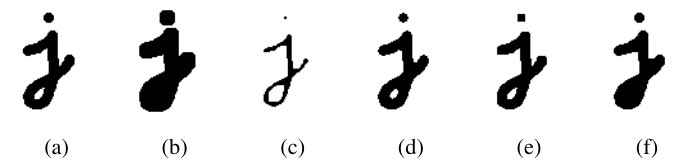
\includegraphics[width = \linewidth]{figs/background/png/binary-image-processing.jpg}
    \caption[A collection of morphological operations on a binary image]{A collection of morphological operations on a binary image: (a) original image; (b) dilation; (c) erosion; (d) majority; (e) opening; (f) closing. Image from \cite{szeliskiComputerVisionAlgorithms2022}}
    \label{fig:binary-image-processing}
\end{figure}

Dilation and erosion represent the two principal operations employed in model-image registration (Equation \ref{eq:dilation-erosion}).
Each of these operations involves a two-step process: initially, a convolution operation is performed on the binary image; subsequently, a threshold is applied to the output of the convolution to decide whether the central pixel will be assigned a value of 0 or 1.
If $f$ denotes the input image, and $s$ symbolizes the convolution kernel of $1$s, and $c=f\otimes s$ indicates the count of $1$s in the convolution output, then dilation and erosion can be expressed mathematically (\cref{eq:dilation-erosion}).

\begin{equation}
    \begin{aligned}
        \text{dilate}(f,s) &= \theta(c,1) \\
        \text{erode}(f,s) &= \theta(c,S) 
    \end{aligned}
    \label{eq:dilation-erosion}
\end{equation}

Where $\theta$ represents a thresholding function.

\begin{equation}
    \theta (f,t) = \begin{cases}
        1 &\text{ if } f\ge t \\
        0 &\text{ else}
    \end{cases}
\end{equation}

%%% Local Variables:
%%% mode: latex
%%% TeX-master: "../../../Andrew_Jensen_Dissertation"
%%% End:
